\documentclass{standalone}
\usepackage{tikz}
\usetikzlibrary{patterns, positioning}

\begin{document}
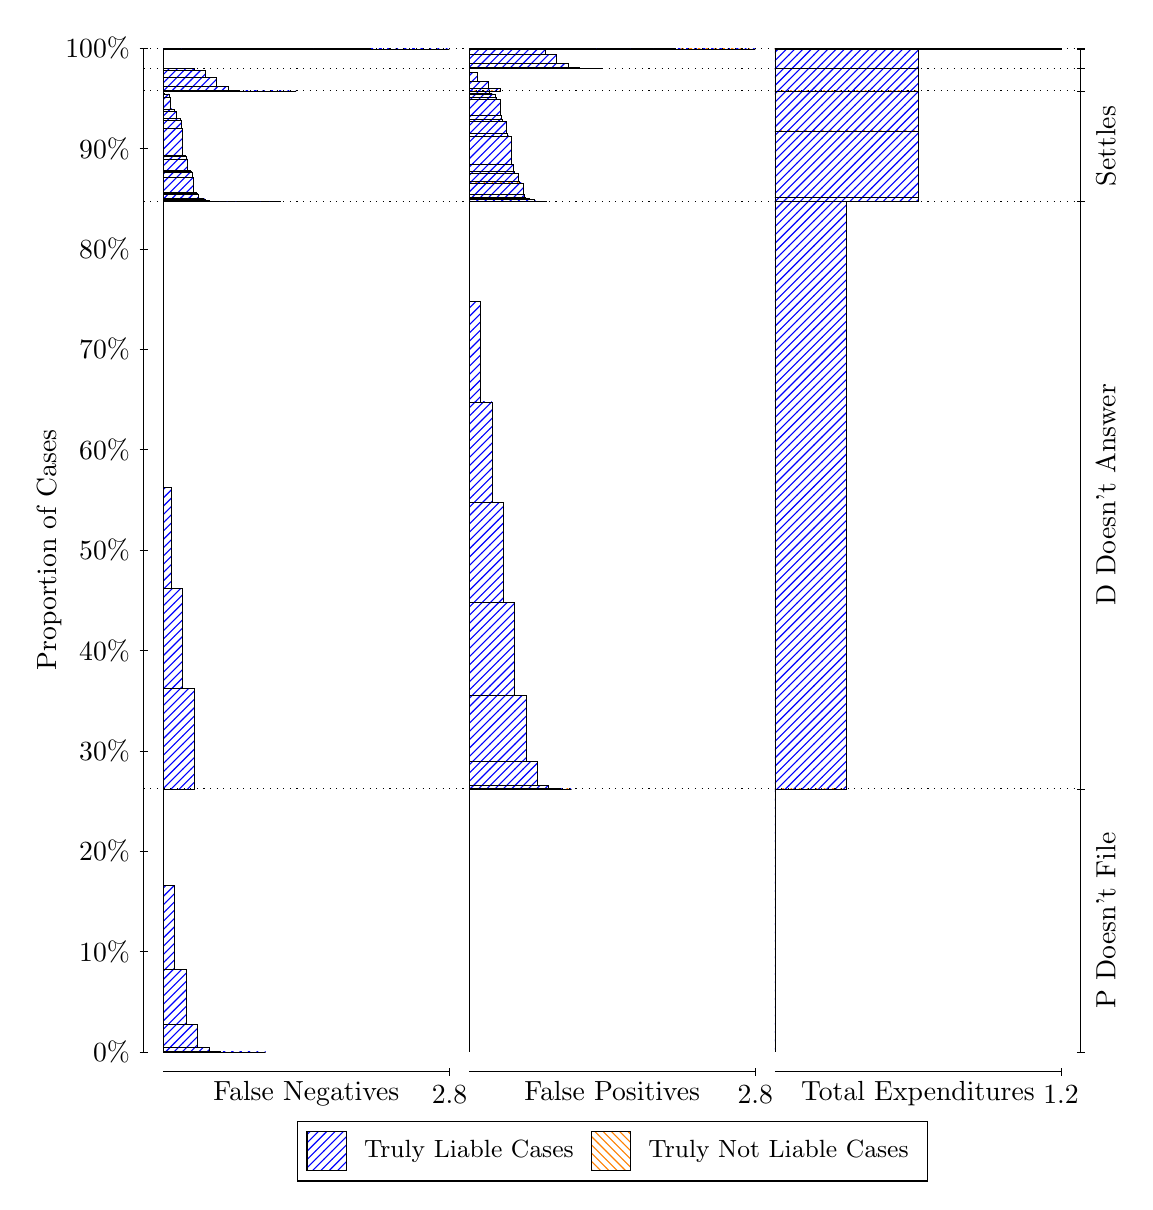
\begin{tikzpicture}
\draw[black, very thin] (1.5,1.75) -- (1.5,14.5);
\node[rotate=90, anchor=center] at (0.3, 8.125) {Proportion of Cases};
\draw[black, very thin] (1.45,1.75) -- (1.55,1.75);
\node[anchor=east] at (1.45, 1.75) {0\%};
\draw[black, very thin] (1.45,3.025) -- (1.55,3.025);
\node[anchor=east] at (1.45, 3.025) {10\%};
\draw[black, very thin] (1.45,4.3) -- (1.55,4.3);
\node[anchor=east] at (1.45, 4.3) {20\%};
\draw[black, very thin] (1.45,5.575) -- (1.55,5.575);
\node[anchor=east] at (1.45, 5.575) {30\%};
\draw[black, very thin] (1.45,6.85) -- (1.55,6.85);
\node[anchor=east] at (1.45, 6.85) {40\%};
\draw[black, very thin] (1.45,8.125) -- (1.55,8.125);
\node[anchor=east] at (1.45, 8.125) {50\%};
\draw[black, very thin] (1.45,9.4) -- (1.55,9.4);
\node[anchor=east] at (1.45, 9.4) {60\%};
\draw[black, very thin] (1.45,10.675) -- (1.55,10.675);
\node[anchor=east] at (1.45, 10.675) {70\%};
\draw[black, very thin] (1.45,11.95) -- (1.55,11.95);
\node[anchor=east] at (1.45, 11.95) {80\%};
\draw[black, very thin] (1.45,13.225) -- (1.55,13.225);
\node[anchor=east] at (1.45, 13.225) {90\%};
\draw[black, very thin] (1.45,14.5) -- (1.55,14.5);
\node[anchor=east] at (1.45, 14.5) {100\%};

\draw[black, very thin] (13.4,1.75) -- (13.4,14.5);
\draw[black, very thin] (13.35,1.75) -- (13.45,1.75);
\node[anchor=west] at (13.35, 1.75) {};
\draw[black, very thin] (13.35,5.0914) -- (13.45,5.0914);
\node[anchor=west] at (13.35, 5.0914) {};
\draw[black, very thin] (13.35,12.555) -- (13.45,12.555);
\node[anchor=west] at (13.35, 12.555) {};
\draw[black, very thin] (13.35,13.957) -- (13.45,13.957);
\node[anchor=west] at (13.35, 13.957) {};
\draw[black, very thin] (13.35,14.245) -- (13.45,14.245);
\node[anchor=west] at (13.35, 14.245) {};
\draw[black, very thin] (13.35,14.489) -- (13.45,14.489);
\node[anchor=west] at (13.35, 14.489) {};
\draw[black, very thin] (13.35,14.5) -- (13.45,14.5);
\node[anchor=west] at (13.35, 14.5) {};

\draw[black, very thin, pattern color=blue, pattern=north east lines] (1.75,1.75) rectangle (3.0476,1.75);
\draw[black, very thin, pattern color=blue, pattern=north east lines] (1.75,1.75) rectangle (2.9034,1.75);
\draw[black, very thin, pattern color=blue, pattern=north east lines] (1.75,1.75) rectangle (2.7593,1.75);
\draw[black, very thin, pattern color=blue, pattern=north east lines] (1.75,1.75) rectangle (2.6151,1.7502);
\draw[black, very thin, pattern color=blue, pattern=north east lines] (1.75,1.7502) rectangle (2.4709,1.7554);
\draw[black, very thin, pattern color=blue, pattern=north east lines] (1.75,1.7554) rectangle (2.3267,1.8131);
\draw[black, very thin, pattern color=blue, pattern=north east lines] (1.75,1.8131) rectangle (2.1825,2.0967);
\draw[black, very thin, pattern color=blue, pattern=north east lines] (1.75,2.0967) rectangle (2.0384,2.8013);
\draw[black, very thin, pattern color=blue, pattern=north east lines] (1.75,2.8013) rectangle (1.8942,3.8676);
\draw[black, very thin, pattern color=orange, pattern=north west lines] (1.75,3.8676) rectangle (1.75,3.8676);
\draw[black, very thin, pattern color=blue, pattern=north east lines] (1.75,3.8676) rectangle (1.75,5.0914);
\draw[black, very thin, pattern color=blue, pattern=north east lines] (1.75,5.0914) rectangle (2.1393,6.3664);
\draw[black, very thin, pattern color=blue, pattern=north east lines] (1.75,6.3664) rectangle (1.9951,7.6414);
\draw[black, very thin, pattern color=blue, pattern=north east lines] (1.75,7.6414) rectangle (1.8509,8.9161);
\draw[black, very thin, pattern color=orange, pattern=north west lines] (1.75,8.9161) rectangle (1.75,8.9161);
\draw[black, very thin, pattern color=blue, pattern=north east lines] (1.75,8.9161) rectangle (1.75,12.555);
\draw[black, very thin, pattern color=blue, pattern=north east lines] (1.75,12.555) rectangle (3.2423,12.555);
\draw[black, very thin, pattern color=blue, pattern=north east lines] (1.75,12.555) rectangle (3.1774,12.555);
\draw[black, very thin, pattern color=blue, pattern=north east lines] (1.75,12.555) rectangle (3.1125,12.555);
\draw[black, very thin, pattern color=blue, pattern=north east lines] (1.75,12.555) rectangle (3.0981,12.555);
\draw[black, very thin, pattern color=blue, pattern=north east lines] (1.75,12.555) rectangle (3.0476,12.555);
\draw[black, very thin, pattern color=blue, pattern=north east lines] (1.75,12.555) rectangle (3.0332,12.555);
\draw[black, very thin, pattern color=blue, pattern=north east lines] (1.75,12.555) rectangle (2.9827,12.555);
\draw[black, very thin, pattern color=blue, pattern=north east lines] (1.75,12.555) rectangle (2.9683,12.555);
\draw[black, very thin, pattern color=blue, pattern=north east lines] (1.75,12.555) rectangle (2.9539,12.555);
\draw[black, very thin, pattern color=blue, pattern=north east lines] (1.75,12.555) rectangle (2.9179,12.555);
\draw[black, very thin, pattern color=blue, pattern=north east lines] (1.75,12.555) rectangle (2.9034,12.555);
\draw[black, very thin, pattern color=blue, pattern=north east lines] (1.75,12.555) rectangle (2.889,12.555);
\draw[black, very thin, pattern color=blue, pattern=north east lines] (1.75,12.555) rectangle (2.853,12.555);
\draw[black, very thin, pattern color=blue, pattern=north east lines] (1.75,12.555) rectangle (2.8386,12.555);
\draw[black, very thin, pattern color=blue, pattern=north east lines] (1.75,12.555) rectangle (2.8241,12.555);
\draw[black, very thin, pattern color=blue, pattern=north east lines] (1.75,12.555) rectangle (2.8097,12.555);
\draw[black, very thin, pattern color=blue, pattern=north east lines] (1.75,12.555) rectangle (2.7737,12.555);
\draw[black, very thin, pattern color=blue, pattern=north east lines] (1.75,12.555) rectangle (2.7593,12.555);
\draw[black, very thin, pattern color=blue, pattern=north east lines] (1.75,12.555) rectangle (2.7448,12.555);
\draw[black, very thin, pattern color=blue, pattern=north east lines] (1.75,12.555) rectangle (2.7088,12.555);
\draw[black, very thin, pattern color=blue, pattern=north east lines] (1.75,12.555) rectangle (2.6944,12.555);
\draw[black, very thin, pattern color=blue, pattern=north east lines] (1.75,12.555) rectangle (2.68,12.555);
\draw[black, very thin, pattern color=blue, pattern=north east lines] (1.75,12.555) rectangle (2.6655,12.555);
\draw[black, very thin, pattern color=blue, pattern=north east lines] (1.75,12.555) rectangle (2.6295,12.555);
\draw[black, very thin, pattern color=blue, pattern=north east lines] (1.75,12.555) rectangle (2.6151,12.555);
\draw[black, very thin, pattern color=blue, pattern=north east lines] (1.75,12.555) rectangle (2.6007,12.555);
\draw[black, very thin, pattern color=blue, pattern=north east lines] (1.75,12.555) rectangle (2.5646,12.555);
\draw[black, very thin, pattern color=blue, pattern=north east lines] (1.75,12.555) rectangle (2.5502,12.555);
\draw[black, very thin, pattern color=blue, pattern=north east lines] (1.75,12.555) rectangle (2.5358,12.555);
\draw[black, very thin, pattern color=blue, pattern=north east lines] (1.75,12.555) rectangle (2.5214,12.555);
\draw[black, very thin, pattern color=blue, pattern=north east lines] (1.75,12.555) rectangle (2.4853,12.555);
\draw[black, very thin, pattern color=blue, pattern=north east lines] (1.75,12.555) rectangle (2.4709,12.555);
\draw[black, very thin, pattern color=blue, pattern=north east lines] (1.75,12.555) rectangle (2.4565,12.555);
\draw[black, very thin, pattern color=blue, pattern=north east lines] (1.75,12.555) rectangle (2.4204,12.556);
\draw[black, very thin, pattern color=blue, pattern=north east lines] (1.75,12.556) rectangle (2.406,12.556);
\draw[black, very thin, pattern color=blue, pattern=north east lines] (1.75,12.556) rectangle (2.3916,12.556);
\draw[black, very thin, pattern color=blue, pattern=north east lines] (1.75,12.556) rectangle (2.3772,12.557);
\draw[black, very thin, pattern color=blue, pattern=north east lines] (1.75,12.557) rectangle (2.3411,12.559);
\draw[black, very thin, pattern color=blue, pattern=north east lines] (1.75,12.559) rectangle (2.3267,12.561);
\draw[black, very thin, pattern color=blue, pattern=north east lines] (1.75,12.561) rectangle (2.3123,12.562);
\draw[black, very thin, pattern color=blue, pattern=north east lines] (1.75,12.562) rectangle (2.2763,12.585);
\draw[black, very thin, pattern color=blue, pattern=north east lines] (1.75,12.585) rectangle (2.2618,12.592);
\draw[black, very thin, pattern color=blue, pattern=north east lines] (1.75,12.592) rectangle (2.2474,12.595);
\draw[black, very thin, pattern color=blue, pattern=north east lines] (1.75,12.595) rectangle (2.233,12.598);
\draw[black, very thin, pattern color=blue, pattern=north east lines] (1.75,12.598) rectangle (2.197,12.643);
\draw[black, very thin, pattern color=blue, pattern=north east lines] (1.75,12.643) rectangle (2.1825,12.66);
\draw[black, very thin, pattern color=blue, pattern=north east lines] (1.75,12.66) rectangle (2.1681,12.664);
\draw[black, very thin, pattern color=blue, pattern=north east lines] (1.75,12.664) rectangle (2.1321,12.86);
\draw[black, very thin, pattern color=blue, pattern=north east lines] (1.75,12.86) rectangle (2.1177,12.919);
\draw[black, very thin, pattern color=blue, pattern=north east lines] (1.75,12.919) rectangle (2.1032,12.938);
\draw[black, very thin, pattern color=blue, pattern=north east lines] (1.75,12.938) rectangle (2.0888,12.944);
\draw[black, very thin, pattern color=blue, pattern=north east lines] (1.75,12.944) rectangle (2.0528,13.093);
\draw[black, very thin, pattern color=blue, pattern=north east lines] (1.75,13.093) rectangle (2.0384,13.128);
\draw[black, very thin, pattern color=blue, pattern=north east lines] (1.75,13.128) rectangle (2.0239,13.133);
\draw[black, very thin, pattern color=blue, pattern=north east lines] (1.75,13.133) rectangle (1.9879,13.483);
\draw[black, very thin, pattern color=blue, pattern=north east lines] (1.75,13.483) rectangle (1.9735,13.582);
\draw[black, very thin, pattern color=blue, pattern=north east lines] (1.75,13.582) rectangle (1.9591,13.604);
\draw[black, very thin, pattern color=blue, pattern=north east lines] (1.75,13.604) rectangle (1.9446,13.608);
\draw[black, very thin, pattern color=blue, pattern=north east lines] (1.75,13.608) rectangle (1.9086,13.703);
\draw[black, very thin, pattern color=blue, pattern=north east lines] (1.75,13.703) rectangle (1.8942,13.725);
\draw[black, very thin, pattern color=blue, pattern=north east lines] (1.75,13.725) rectangle (1.8798,13.726);
\draw[black, very thin, pattern color=blue, pattern=north east lines] (1.75,13.726) rectangle (1.8437,13.875);
\draw[black, very thin, pattern color=blue, pattern=north east lines] (1.75,13.875) rectangle (1.8293,13.911);
\draw[black, very thin, pattern color=blue, pattern=north east lines] (1.75,13.911) rectangle (1.8149,13.917);
\draw[black, very thin, pattern color=blue, pattern=north east lines] (1.75,13.917) rectangle (1.7644,13.931);
\draw[black, very thin, pattern color=orange, pattern=north west lines] (1.75,13.931) rectangle (1.75,13.931);
\draw[black, very thin, pattern color=blue, pattern=north east lines] (1.75,13.931) rectangle (1.75,13.957);
\draw[black, very thin, pattern color=blue, pattern=north east lines] (1.75,13.957) rectangle (3.4369,13.957);
\draw[black, very thin, pattern color=blue, pattern=north east lines] (1.75,13.957) rectangle (3.2927,13.957);
\draw[black, very thin, pattern color=blue, pattern=north east lines] (1.75,13.957) rectangle (3.1485,13.957);
\draw[black, very thin, pattern color=blue, pattern=north east lines] (1.75,13.957) rectangle (3.0044,13.957);
\draw[black, very thin, pattern color=blue, pattern=north east lines] (1.75,13.957) rectangle (2.8602,13.957);
\draw[black, very thin, pattern color=blue, pattern=north east lines] (1.75,13.957) rectangle (2.716,13.961);
\draw[black, very thin, pattern color=blue, pattern=north east lines] (1.75,13.961) rectangle (2.5718,14.01);
\draw[black, very thin, pattern color=blue, pattern=north east lines] (1.75,14.01) rectangle (2.4276,14.129);
\draw[black, very thin, pattern color=blue, pattern=north east lines] (1.75,14.129) rectangle (2.2835,14.216);
\draw[black, very thin, pattern color=blue, pattern=north east lines] (1.75,14.216) rectangle (2.1393,14.245);
\draw[black, very thin, pattern color=orange, pattern=north west lines] (1.75,14.245) rectangle (1.75,14.245);
\draw[black, very thin, pattern color=blue, pattern=north east lines] (1.75,14.245) rectangle (2.1393,14.245);
\draw[black, very thin, pattern color=blue, pattern=north east lines] (1.75,14.245) rectangle (1.9951,14.245);
\draw[black, very thin, pattern color=blue, pattern=north east lines] (1.75,14.245) rectangle (1.8509,14.246);
\draw[black, very thin, pattern color=orange, pattern=north west lines] (1.75,14.246) rectangle (1.75,14.246);
\draw[black, very thin, pattern color=blue, pattern=north east lines] (1.75,14.246) rectangle (1.75,14.489);
\draw[black, very thin, pattern color=blue, pattern=north east lines] (1.75,14.489) rectangle (5.3833,14.489);
\draw[black, very thin, pattern color=blue, pattern=north east lines] (1.75,14.489) rectangle (5.2392,14.489);
\draw[black, very thin, pattern color=blue, pattern=north east lines] (1.75,14.489) rectangle (5.095,14.489);
\draw[black, very thin, pattern color=blue, pattern=north east lines] (1.75,14.489) rectangle (4.9508,14.489);
\draw[black, very thin, pattern color=blue, pattern=north east lines] (1.75,14.489) rectangle (4.9508,14.489);
\draw[black, very thin, pattern color=blue, pattern=north east lines] (1.75,14.489) rectangle (4.8066,14.489);
\draw[black, very thin, pattern color=blue, pattern=north east lines] (1.75,14.489) rectangle (4.6624,14.489);
\draw[black, very thin, pattern color=blue, pattern=north east lines] (1.75,14.489) rectangle (4.6624,14.489);
\draw[black, very thin, pattern color=blue, pattern=north east lines] (1.75,14.489) rectangle (4.5183,14.489);
\draw[black, very thin, pattern color=blue, pattern=north east lines] (1.75,14.489) rectangle (4.5183,14.489);
\draw[black, very thin, pattern color=blue, pattern=north east lines] (1.75,14.489) rectangle (4.3741,14.491);
\draw[black, very thin, pattern color=blue, pattern=north east lines] (1.75,14.491) rectangle (4.2299,14.491);
\draw[black, very thin, pattern color=blue, pattern=north east lines] (1.75,14.491) rectangle (4.2299,14.492);
\draw[black, very thin, pattern color=blue, pattern=north east lines] (1.75,14.492) rectangle (4.0857,14.493);
\draw[black, very thin, pattern color=blue, pattern=north east lines] (1.75,14.493) rectangle (3.9415,14.493);
\draw[black, very thin, pattern color=blue, pattern=north east lines] (1.75,14.493) rectangle (3.7974,14.493);
\draw[black, very thin, pattern color=blue, pattern=north east lines] (1.75,14.493) rectangle (3.7974,14.493);
\draw[black, very thin, pattern color=blue, pattern=north east lines] (1.75,14.493) rectangle (3.6532,14.493);
\draw[black, very thin, pattern color=blue, pattern=north east lines] (1.75,14.493) rectangle (2.1249,14.493);
\draw[black, very thin, pattern color=blue, pattern=north east lines] (1.75,14.493) rectangle (1.9807,14.493);
\draw[black, very thin, pattern color=blue, pattern=north east lines] (1.75,14.493) rectangle (1.8365,14.493);
\draw[black, very thin, pattern color=blue, pattern=north east lines] (1.75,14.493) rectangle (1.8365,14.493);
\draw[black, very thin, pattern color=orange, pattern=north west lines] (1.75,14.493) rectangle (1.75,14.493);
\draw[black, very thin, pattern color=blue, pattern=north east lines] (1.75,14.493) rectangle (1.75,14.5);
\draw[black, very thin, pattern color=orange, pattern=north west lines] (5.6333,1.75) rectangle (5.6333,1.75);
\draw[black, very thin, pattern color=blue, pattern=north east lines] (5.6333,1.75) rectangle (5.6333,5.0914);
\draw[black, very thin, pattern color=orange, pattern=north west lines] (5.6333,5.0914) rectangle (6.931,5.0914);
\draw[black, very thin, pattern color=blue, pattern=north east lines] (5.6333,5.0914) rectangle (6.931,5.0914);
\draw[black, very thin, pattern color=blue, pattern=north east lines] (5.6333,5.0914) rectangle (6.7868,5.0928);
\draw[black, very thin, pattern color=blue, pattern=north east lines] (5.6333,5.0928) rectangle (6.6426,5.1312);
\draw[black, very thin, pattern color=blue, pattern=north east lines] (5.6333,5.1312) rectangle (6.4984,5.4371);
\draw[black, very thin, pattern color=blue, pattern=north east lines] (5.6333,5.4371) rectangle (6.3542,6.2788);
\draw[black, very thin, pattern color=blue, pattern=north east lines] (5.6333,6.2788) rectangle (6.2101,7.4638);
\draw[black, very thin, pattern color=blue, pattern=north east lines] (5.6333,7.4638) rectangle (6.0659,8.7307);
\draw[black, very thin, pattern color=blue, pattern=north east lines] (5.6333,8.7307) rectangle (5.9217,10.005);
\draw[black, very thin, pattern color=blue, pattern=north east lines] (5.6333,10.005) rectangle (5.7775,11.28);
\draw[black, very thin, pattern color=blue, pattern=north east lines] (5.6333,11.28) rectangle (5.6333,12.555);
\draw[black, very thin, pattern color=orange, pattern=north west lines] (5.6333,12.555) rectangle (6.6065,12.555);
\draw[black, very thin, pattern color=blue, pattern=north east lines] (5.6333,12.555) rectangle (6.6065,12.556);
\draw[black, very thin, pattern color=orange, pattern=north west lines] (5.6333,12.556) rectangle (6.5417,12.556);
\draw[black, very thin, pattern color=blue, pattern=north east lines] (5.6333,12.556) rectangle (6.5417,12.557);
\draw[black, very thin, pattern color=orange, pattern=north west lines] (5.6333,12.557) rectangle (6.4768,12.557);
\draw[black, very thin, pattern color=blue, pattern=north east lines] (5.6333,12.557) rectangle (6.4768,12.56);
\draw[black, very thin, pattern color=blue, pattern=north east lines] (5.6333,12.56) rectangle (6.4624,12.577);
\draw[black, very thin, pattern color=orange, pattern=north west lines] (5.6333,12.577) rectangle (6.4119,12.577);
\draw[black, very thin, pattern color=blue, pattern=north east lines] (5.6333,12.577) rectangle (6.4119,12.581);
\draw[black, very thin, pattern color=blue, pattern=north east lines] (5.6333,12.581) rectangle (6.3975,12.595);
\draw[black, very thin, pattern color=orange, pattern=north west lines] (5.6333,12.595) rectangle (6.347,12.595);
\draw[black, very thin, pattern color=blue, pattern=north east lines] (5.6333,12.595) rectangle (6.347,12.601);
\draw[black, very thin, pattern color=blue, pattern=north east lines] (5.6333,12.601) rectangle (6.3326,12.637);
\draw[black, very thin, pattern color=blue, pattern=north east lines] (5.6333,12.637) rectangle (6.3182,12.786);
\draw[black, very thin, pattern color=orange, pattern=north west lines] (5.6333,12.786) rectangle (6.2821,12.786);
\draw[black, very thin, pattern color=blue, pattern=north east lines] (5.6333,12.786) rectangle (6.2821,12.787);
\draw[black, very thin, pattern color=blue, pattern=north east lines] (5.6333,12.787) rectangle (6.2677,12.809);
\draw[black, very thin, pattern color=blue, pattern=north east lines] (5.6333,12.809) rectangle (6.2533,12.904);
\draw[black, very thin, pattern color=orange, pattern=north west lines] (5.6333,12.904) rectangle (6.2173,12.904);
\draw[black, very thin, pattern color=blue, pattern=north east lines] (5.6333,12.904) rectangle (6.2173,12.908);
\draw[black, very thin, pattern color=blue, pattern=north east lines] (5.6333,12.908) rectangle (6.2028,12.93);
\draw[black, very thin, pattern color=blue, pattern=north east lines] (5.6333,12.93) rectangle (6.1884,13.029);
\draw[black, very thin, pattern color=blue, pattern=north east lines] (5.6333,13.029) rectangle (6.174,13.379);
\draw[black, very thin, pattern color=blue, pattern=north east lines] (5.6333,13.379) rectangle (6.138,13.384);
\draw[black, very thin, pattern color=blue, pattern=north east lines] (5.6333,13.384) rectangle (6.1235,13.419);
\draw[black, very thin, pattern color=blue, pattern=north east lines] (5.6333,13.419) rectangle (6.1091,13.568);
\draw[black, very thin, pattern color=blue, pattern=north east lines] (5.6333,13.568) rectangle (6.0731,13.574);
\draw[black, very thin, pattern color=blue, pattern=north east lines] (5.6333,13.574) rectangle (6.0587,13.593);
\draw[black, very thin, pattern color=blue, pattern=north east lines] (5.6333,13.593) rectangle (6.0442,13.652);
\draw[black, very thin, pattern color=blue, pattern=north east lines] (5.6333,13.652) rectangle (6.0298,13.848);
\draw[black, very thin, pattern color=blue, pattern=north east lines] (5.6333,13.848) rectangle (5.9938,13.852);
\draw[black, very thin, pattern color=blue, pattern=north east lines] (5.6333,13.852) rectangle (5.9794,13.869);
\draw[black, very thin, pattern color=blue, pattern=north east lines] (5.6333,13.869) rectangle (5.9649,13.914);
\draw[black, very thin, pattern color=blue, pattern=north east lines] (5.6333,13.914) rectangle (5.9289,13.917);
\draw[black, very thin, pattern color=blue, pattern=north east lines] (5.6333,13.917) rectangle (5.9145,13.92);
\draw[black, very thin, pattern color=blue, pattern=north east lines] (5.6333,13.92) rectangle (5.9001,13.927);
\draw[black, very thin, pattern color=blue, pattern=north east lines] (5.6333,13.927) rectangle (5.8856,13.95);
\draw[black, very thin, pattern color=blue, pattern=north east lines] (5.6333,13.95) rectangle (5.8496,13.951);
\draw[black, very thin, pattern color=blue, pattern=north east lines] (5.6333,13.951) rectangle (5.8352,13.953);
\draw[black, very thin, pattern color=blue, pattern=north east lines] (5.6333,13.953) rectangle (5.8208,13.955);
\draw[black, very thin, pattern color=blue, pattern=north east lines] (5.6333,13.955) rectangle (5.7847,13.956);
\draw[black, very thin, pattern color=blue, pattern=north east lines] (5.6333,13.956) rectangle (5.7703,13.956);
\draw[black, very thin, pattern color=blue, pattern=north east lines] (5.6333,13.956) rectangle (5.7559,13.956);
\draw[black, very thin, pattern color=blue, pattern=north east lines] (5.6333,13.956) rectangle (5.7415,13.956);
\draw[black, very thin, pattern color=blue, pattern=north east lines] (5.6333,13.956) rectangle (5.7054,13.957);
\draw[black, very thin, pattern color=blue, pattern=north east lines] (5.6333,13.957) rectangle (5.691,13.957);
\draw[black, very thin, pattern color=blue, pattern=north east lines] (5.6333,13.957) rectangle (5.6766,13.957);
\draw[black, very thin, pattern color=blue, pattern=north east lines] (5.6333,13.957) rectangle (5.6405,13.957);
\draw[black, very thin, pattern color=blue, pattern=north east lines] (5.6333,13.957) rectangle (5.6333,13.957);
\draw[black, very thin, pattern color=orange, pattern=north west lines] (5.6333,13.957) rectangle (6.0226,13.957);
\draw[black, very thin, pattern color=blue, pattern=north east lines] (5.6333,13.957) rectangle (6.0226,13.986);
\draw[black, very thin, pattern color=blue, pattern=north east lines] (5.6333,13.986) rectangle (5.8784,14.073);
\draw[black, very thin, pattern color=blue, pattern=north east lines] (5.6333,14.073) rectangle (5.7343,14.192);
\draw[black, very thin, pattern color=blue, pattern=north east lines] (5.6333,14.192) rectangle (5.6333,14.245);
\draw[black, very thin, pattern color=orange, pattern=north west lines] (5.6333,14.245) rectangle (7.3202,14.245);
\draw[black, very thin, pattern color=blue, pattern=north east lines] (5.6333,14.245) rectangle (7.3202,14.245);
\draw[black, very thin, pattern color=blue, pattern=north east lines] (5.6333,14.245) rectangle (7.1761,14.246);
\draw[black, very thin, pattern color=blue, pattern=north east lines] (5.6333,14.246) rectangle (7.0319,14.251);
\draw[black, very thin, pattern color=blue, pattern=north east lines] (5.6333,14.251) rectangle (6.8877,14.304);
\draw[black, very thin, pattern color=blue, pattern=north east lines] (5.6333,14.304) rectangle (6.7435,14.423);
\draw[black, very thin, pattern color=blue, pattern=north east lines] (5.6333,14.423) rectangle (6.5993,14.481);
\draw[black, very thin, pattern color=blue, pattern=north east lines] (5.6333,14.481) rectangle (6.4552,14.489);
\draw[black, very thin, pattern color=blue, pattern=north east lines] (5.6333,14.489) rectangle (6.311,14.489);
\draw[black, very thin, pattern color=blue, pattern=north east lines] (5.6333,14.489) rectangle (6.1668,14.489);
\draw[black, very thin, pattern color=blue, pattern=north east lines] (5.6333,14.489) rectangle (6.0226,14.489);
\draw[black, very thin, pattern color=orange, pattern=north west lines] (5.6333,14.489) rectangle (9.2667,14.489);
\draw[black, very thin, pattern color=blue, pattern=north east lines] (5.6333,14.489) rectangle (9.2667,14.489);
\draw[black, very thin, pattern color=orange, pattern=north west lines] (5.6333,14.489) rectangle (9.1225,14.489);
\draw[black, very thin, pattern color=blue, pattern=north east lines] (5.6333,14.489) rectangle (9.1225,14.489);
\draw[black, very thin, pattern color=orange, pattern=north west lines] (5.6333,14.489) rectangle (8.9783,14.489);
\draw[black, very thin, pattern color=blue, pattern=north east lines] (5.6333,14.489) rectangle (8.9783,14.489);
\draw[black, very thin, pattern color=orange, pattern=north west lines] (5.6333,14.489) rectangle (8.8341,14.489);
\draw[black, very thin, pattern color=blue, pattern=north east lines] (5.6333,14.489) rectangle (8.8341,14.489);
\draw[black, very thin, pattern color=orange, pattern=north west lines] (5.6333,14.489) rectangle (8.6899,14.489);
\draw[black, very thin, pattern color=blue, pattern=north east lines] (5.6333,14.489) rectangle (8.6899,14.489);
\draw[black, very thin, pattern color=orange, pattern=north west lines] (5.6333,14.489) rectangle (8.5458,14.489);
\draw[black, very thin, pattern color=blue, pattern=north east lines] (5.6333,14.489) rectangle (8.5458,14.489);
\draw[black, very thin, pattern color=blue, pattern=north east lines] (5.6333,14.489) rectangle (8.5458,14.489);
\draw[black, very thin, pattern color=orange, pattern=north west lines] (5.6333,14.489) rectangle (8.4016,14.489);
\draw[black, very thin, pattern color=blue, pattern=north east lines] (5.6333,14.489) rectangle (8.4016,14.489);
\draw[black, very thin, pattern color=blue, pattern=north east lines] (5.6333,14.489) rectangle (8.4016,14.49);
\draw[black, very thin, pattern color=orange, pattern=north west lines] (5.6333,14.49) rectangle (8.2574,14.49);
\draw[black, very thin, pattern color=blue, pattern=north east lines] (5.6333,14.49) rectangle (8.2574,14.49);
\draw[black, very thin, pattern color=blue, pattern=north east lines] (5.6333,14.49) rectangle (8.2574,14.491);
\draw[black, very thin, pattern color=blue, pattern=north east lines] (5.6333,14.491) rectangle (8.1132,14.492);
\draw[black, very thin, pattern color=orange, pattern=north west lines] (5.6333,14.492) rectangle (8.1132,14.492);
\draw[black, very thin, pattern color=blue, pattern=north east lines] (5.6333,14.492) rectangle (8.1132,14.492);
\draw[black, very thin, pattern color=blue, pattern=north east lines] (5.6333,14.492) rectangle (8.1132,14.493);
\draw[black, very thin, pattern color=blue, pattern=north east lines] (5.6333,14.493) rectangle (7.969,14.495);
\draw[black, very thin, pattern color=blue, pattern=north east lines] (5.6333,14.495) rectangle (7.969,14.495);
\draw[black, very thin, pattern color=blue, pattern=north east lines] (5.6333,14.495) rectangle (7.969,14.495);
\draw[black, very thin, pattern color=blue, pattern=north east lines] (5.6333,14.495) rectangle (7.8249,14.496);
\draw[black, very thin, pattern color=blue, pattern=north east lines] (5.6333,14.496) rectangle (7.8249,14.496);
\draw[black, very thin, pattern color=blue, pattern=north east lines] (5.6333,14.496) rectangle (7.6807,14.496);
\draw[black, very thin, pattern color=blue, pattern=north east lines] (5.6333,14.496) rectangle (7.6807,14.496);
\draw[black, very thin, pattern color=blue, pattern=north east lines] (5.6333,14.496) rectangle (7.6807,14.496);
\draw[black, very thin, pattern color=blue, pattern=north east lines] (5.6333,14.496) rectangle (7.5365,14.496);
\draw[black, very thin, pattern color=blue, pattern=north east lines] (5.6333,14.496) rectangle (7.5365,14.496);
\draw[black, very thin, pattern color=blue, pattern=north east lines] (5.6333,14.496) rectangle (7.5365,14.496);
\draw[black, very thin, pattern color=blue, pattern=north east lines] (5.6333,14.496) rectangle (7.3923,14.496);
\draw[black, very thin, pattern color=blue, pattern=north east lines] (5.6333,14.496) rectangle (7.3923,14.496);
\draw[black, very thin, pattern color=blue, pattern=north east lines] (5.6333,14.496) rectangle (7.3923,14.496);
\draw[black, very thin, pattern color=blue, pattern=north east lines] (5.6333,14.496) rectangle (7.2481,14.496);
\draw[black, very thin, pattern color=blue, pattern=north east lines] (5.6333,14.496) rectangle (7.104,14.496);
\draw[black, very thin, pattern color=blue, pattern=north east lines] (5.6333,14.496) rectangle (6.9598,14.496);
\draw[black, very thin, pattern color=blue, pattern=north east lines] (5.6333,14.496) rectangle (6.8156,14.496);
\draw[black, very thin, pattern color=orange, pattern=north west lines] (5.6333,14.496) rectangle (5.6333,14.496);
\draw[black, very thin, pattern color=blue, pattern=north east lines] (5.6333,14.496) rectangle (5.6333,14.5);
\draw[black, very thin, pattern color=orange, pattern=north west lines] (9.5167,1.75) rectangle (9.5167,1.75);
\draw[black, very thin, pattern color=blue, pattern=north east lines] (9.5167,1.75) rectangle (9.5167,5.0914);
\draw[black, very thin, pattern color=orange, pattern=north west lines] (9.5167,5.0914) rectangle (10.425,5.0914);
\draw[black, very thin, pattern color=blue, pattern=north east lines] (9.5167,5.0914) rectangle (10.425,12.555);
\draw[black, very thin, pattern color=orange, pattern=north west lines] (9.5167,12.555) rectangle (11.333,12.555);
\draw[black, very thin, pattern color=blue, pattern=north east lines] (9.5167,12.555) rectangle (11.333,12.605);
\draw[black, very thin, pattern color=orange, pattern=north west lines] (9.5167,12.605) rectangle (11.333,12.605);
\draw[black, very thin, pattern color=blue, pattern=north east lines] (9.5167,12.605) rectangle (11.333,13.447);
\draw[black, very thin, pattern color=orange, pattern=north west lines] (9.5167,13.447) rectangle (11.333,13.447);
\draw[black, very thin, pattern color=blue, pattern=north east lines] (9.5167,13.447) rectangle (11.333,13.957);
\draw[black, very thin, pattern color=orange, pattern=north west lines] (9.5167,13.957) rectangle (11.333,13.957);
\draw[black, very thin, pattern color=blue, pattern=north east lines] (9.5167,13.957) rectangle (11.333,14.245);
\draw[black, very thin, pattern color=orange, pattern=north west lines] (9.5167,14.245) rectangle (11.333,14.245);
\draw[black, very thin, pattern color=blue, pattern=north east lines] (9.5167,14.245) rectangle (11.333,14.489);
\draw[black, very thin, pattern color=orange, pattern=north west lines] (9.5167,14.489) rectangle (13.15,14.489);
\draw[black, very thin, pattern color=blue, pattern=north east lines] (9.5167,14.489) rectangle (13.15,14.491);
\draw[black, very thin, pattern color=orange, pattern=north west lines] (9.5167,14.491) rectangle (13.15,14.491);
\draw[black, very thin, pattern color=blue, pattern=north east lines] (9.5167,14.491) rectangle (13.15,14.494);
\draw[black, very thin, pattern color=orange, pattern=north west lines] (9.5167,14.494) rectangle (13.15,14.494);
\draw[black, very thin, pattern color=blue, pattern=north east lines] (9.5167,14.494) rectangle (13.15,14.5);
\draw[black, dotted] (1.5,5.0914) -- (13.4,5.0914);
\draw[black, dotted] (1.5,12.555) -- (13.4,12.555);
\draw[black, dotted] (1.5,13.957) -- (13.4,13.957);
\draw[black, dotted] (1.5,14.245) -- (13.4,14.245);
\draw[black, dotted] (1.5,14.489) -- (13.4,14.489);
\draw[black, very thin] (1.75,1.5) -- (5.3833,1.5);
\node[anchor=north] at (3.5667, 1.5) {False Negatives};
\draw[black, very thin] (5.3833,1.45) -- (5.3833,1.55);
\node[anchor=north] at (5.3833, 1.45) {2.8};

\draw[black, very thin] (5.6333,1.5) -- (9.2667,1.5);
\node[anchor=north] at (7.45, 1.5) {False Positives};
\draw[black, very thin] (9.2667,1.45) -- (9.2667,1.55);
\node[anchor=north] at (9.2667, 1.45) {2.8};

\draw[black, very thin] (9.5167,1.5) -- (13.15,1.5);
\node[anchor=north] at (11.333, 1.5) {Total Expenditures};
\draw[black, very thin] (13.15,1.45) -- (13.15,1.55);
\node[anchor=north] at (13.15, 1.45) {1.2};

\node[black, centered, rotate=90] at (13.72, 3.4207) {P Doesn't File};
\node[black, centered, rotate=90] at (13.72, 8.8234) {D Doesn't Answer};
\node[black, centered, rotate=90] at (13.72, 13.256) {Settles};




\draw (7.449999999999999,1.5) node[draw=none] (baseCoordinate) {};
\begin{scope}[align=center]
        \matrix[scale=0.5, draw=black, below=0.5cm of baseCoordinate, nodes={draw}, column sep=0.1cm]{
            \node[rectangle, draw, minimum width=0.5cm, minimum height=0.5cm, pattern=north east lines, pattern color=blue] {}; &
            \node[draw=none, font=\small] (B) {Truly Liable Cases}; &
            \node[rectangle, draw, minimum width=0.5cm, minimum height=0.5cm, pattern=north west lines, pattern color=orange] {}; &
            \node[draw=none, font=\small] (B) {Truly Not Liable Cases}; \\
            };
\end{scope}

\end{tikzpicture}
\end{document}